\documentclass[10pt]{beamer}

%\usepackage[backend=bibtex,firstinits=true,style=verbose-inote,citestyle=authortitle]{biblatex}
\usepackage{bm}
\usepackage{graphicx}
\usepackage{subcaption}
\usepackage{amsmath}
\usepackage{makecell}
\usepackage{filecontents}
\usepackage{biblatex}
\newcommand{\expect}[2][]{
\ifthenelse{\equal{#1}{}}{
\mathbb{E}\left[#2\right]
}{
\underset{#1}{\mathbb{E}}\left[#2\right]
}}

\newcommand{\cov}[2][]{
\ifthenelse{\equal{#1}{}}{
\text{Cov}\left[#2\right]
}{
\underset{#1}{\text{Cov}}\left[#2\right]
}}


\newcommand{\var}[2][]{
\ifthenelse{\equal{#1}{}}{
\text{Var}[#2]
}{
\underset{#1}{\text{Var}}[#2]
}}

\newcommand{\loss}[2][]{
\ifthenelse{\equal{#1}{}}{
\mathcal{L}(#2)
}{
\mathcal{L}_{#1}(#2)
}}

\newcommand{\kl}[2]{
\text{D}_\text{KL}[#1 \parallel #2]
}

\newcommand{\R}{\mathbb{R}}
%\newcommand{\Prob}{\mathbb{P}}

\newcommand{\1}[1]{\mathds{1}\{#1\}}


%\usecolortheme{dolphin}
\setbeamertemplate{navigation symbols}{}
\setbeamertemplate{section in toc}{\inserttocsectionnumber.~\inserttocsection}

\begin{filecontents*}{references.bib}
@incollection{DGR,
title = {Continual Learning with Deep Generative Replay},
author = {Shin, Hanul and Lee, Jung Kwon and Kim, Jaehong and Kim, Jiwon},
booktitle = {Advances in Neural Information Processing Systems 30},
editor = {I. Guyon and U. V. Luxburg and S. Bengio and H. Wallach and R. Fergus and S. Vishwanathan and R. Garnett},
pages = {2990--2999},
year = {2017},
publisher = {Curran Associates, Inc.},
url = {http://papers.nips.cc/paper/6892-continual-learning-with-deep-generative-replay.pdf}
}
@incollection{MeRGAN,
title = {Memory Replay GANs: Learning to Generate New Categories without Forgetting},
author = {Wu, Chenshen and Herranz, Luis and Liu, Xialei and wang, yaxing and van de Weijer, Joost and Raducanu, Bogdan},
booktitle = {Advances in Neural Information Processing Systems 31},
editor = {S. Bengio and H. Wallach and H. Larochelle and K. Grauman and N. Cesa-Bianchi and R. Garnett},
pages = {5962--5972},
year = {2018},
publisher = {Curran Associates, Inc.},
url = {http://papers.nips.cc/paper/7836-memory-replay-gans-learning-to-generate-new-categories-without-forgetting.pdf}
}
@inproceedings{
  CL_with_hypernetworks,
  title={Continual learning with hypernetworks},
  author={Johannes von Oswald and Christian Henning and João Sacramento and Benjamin F. Grewe},
  booktitle={International Conference on Learning Representations},
  year={2020},
  url={https://openreview.net/forum?id=SJgwNerKvB}
}
\end{filecontents*}

\addbibresource{references.bib}


\title{Continual learning with Hypernetworks}
%\subtitle{}
%\author{Ivan Skorokhodov}
%\date{}
%\logo{
\includegraphics[height=1cm]{images/ipavlov-logo.png}}

\newcommand{\citepaper}[1]{\citetitle{#1} by \citeauthor{#1}}

%\graphicspath{{./images}}

%\usetheme{lucid}
\begin{document}

%\begin{frame}
%    \titlepage
%\end{frame}

\section{Model description}
\begin{frame}
    \frametitle{Model description}
    
    \begin{itemize}
        \item A hypernetwork (meta-model) is just a model which produces the weights for some other model.
        \item What is an input to a meta-model? Task input data, task embeddings, random noise, etc.
        \item A meta-model can have less parameters than a target model!
        \item A good way to reduce number of parameters for a meta-model is to condition it on a layer embedding.
    \end{itemize}
    
    \begin{figure}
        \centering
        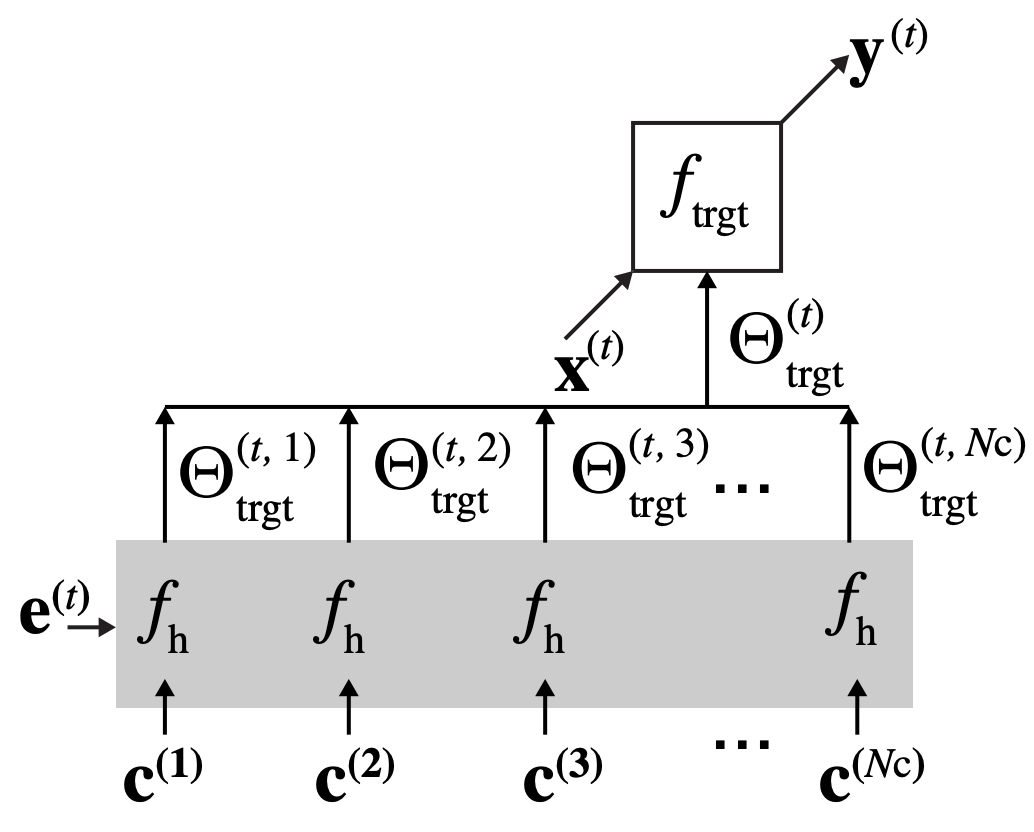
\includegraphics[width=0.5\textwidth]{images/chuncked-hypernetwork.png}
    \end{figure}
\end{frame}

\section{How to use hypernetworks not to forget previous tasks}
\begin{frame}
    \frametitle{How to use hypernetworks not to forget previous tasks}
    
    \begin{itemize}
        \item Condition a hypernetwork on task embedding $e_t$.
        \item Add a regularization term that ensures that its outputs on previously learned task embeddings do not change:
    \end{itemize}
    
    \begin{equation*}
        \mathcal{L}(\theta) = \mathcal{L}^s_\text{cls}(\theta) + \beta \sum_{t=1}^T \| h(\theta_\text{old}, e_t) - h(\theta + \Delta \theta, e_t) \|_2^2,
    \end{equation*}
    where:
    \begin{itemize}
        \item $\mathcal{L}_\text{cls}$ is our classification loss at the current task $t = s$;
        \item $h$ is our hypernetwork;
        \item $\theta$ is the current parameter vector of $h$;
        \item $\Delta \theta$ is the change in parameters produced by Adam optimizer to minimize $\mathcal{L}_\text{cls}$.
        \item $\theta_\text{old}$ --- parameters snapshot before starting to learn the current task.
    \end{itemize}
\end{frame}


\begin{frame}
    \frametitle{CL setups}
    Authors consider 3 different scenarios for continual learning:
    
    \begin{itemize}
        \item With knowing task identities;
        \item Without knowing task identities with a multi-headed model;
        \item Without knowing task identities with a single-headed model.
    \end{itemize}
    
    And they propose two ways to infer a task identity:
    \begin{itemize}
        \item Check which task embedding gives the lowest entropy;
        \item Train a generative memory model and be ready to classify without task identity (in a multi-headed variant);
        \item Train a generative memory and a model that predicts task identity by an input (in a single-headed variant).
    \end{itemize}
\end{frame}


\begin{frame}
    \frametitle{Details, results and discussion}
    \begin{itemize}
        \item Learned task embeddings tend to have a good performance for all the previous tasks as well.
        \item Authors use a VAE model for their generative memory model (people usually use GANs).
        \item They compare the approach to EWC, SI and DGR (these are from 2017), beat them and claim SotA.
        \item A drawback of the approach is the necessity to recompute parameters for all the previous target models on each iteration.
    \end{itemize}
\end{frame}


\end{document}
